
\de{ĐỀ THI HỌC KỲ I NĂM HỌC 2022-2023}{THPT Chuyên Lê Quý Đôn - Quảng Trị}
\begin{center}
	\textbf{PHẦN 1 - TRẮC NGHIỆM}
\end{center}
\Opensolutionfile{ans}[ans/ans]
\begin{ex}%[Dự án đề kiểm tra HKII NH22-23- Hieu PHan]%[THPT Chuyên Lê Quý Đôn - Quảng Trị]%[0D2Y1-2]
     Miền nghiệm của bất phương trình $2 x+y>1$ không chứa điểm nào sau đây?
    \choice
     {$A(1 ; 1)$}
   {$B(2 ; 2)$}
    {$C(3 ; 3)$}
    {\True $D(-1 ;-1)$}
    \loigiai
    {
      Thế tọa độ điểm $D(-1 ;-1)$ vào bất phương trình ta có $2(-1)-1>-1$ (không thỏa).\\
      Vậy $D(-1 ;-1)$ không thuộc miền nghiệm của $2 x+y>1$.
    }
\end{ex}

\begin{ex}%[Dự án đề kiểm tra HKII NH22-23- Hieu PHan]%[THPT Chuyên Lê Quý Đôn - Quảng Trị]%[0H5Y1-2]
    Gọi $M, N$ lần lượt là trung điểm của các cạnh $A B, A C$ của tam giác $A B C$. Hỏi cặp véc-tơ nào sau đây cùng hướng?
    \choice
 { $\overrightarrow{M A}$ và $\overrightarrow{M B}$}
  {$\overrightarrow{M N}$ và $\overrightarrow{C B}$}
  {\True $\overrightarrow{A B}$ và $\overrightarrow{M B}$}
  {$\overrightarrow{A N}$ và $\overrightarrow{C A}$}
    \loigiai
    {
        \immini
        {
 Ta có $\overrightarrow{A B}$ và $\overrightarrow{M B}$ là hai véc-tơ cùng hướng.
        }
        {
              \begin{tikzpicture}[>=stealth,line join=round,line cap=round,line width=0.6pt,font=\footnotesize,scale=0.7]
                \coordinate[label=below left:$B$](B) at (0,0);
                \coordinate[label=below right:$C$](C) at (4,0);
                \coordinate[label=above left:$A$](A) at (1,3);
                \coordinate[label= left:$M$] (M) at ($(B)!0.5!(A)$);
                \coordinate[label=right:$N$](N) at ($(A)!0.5!(C)$);
                \draw (A)--(B)--(C)--cycle;
                \fill (A) circle (1.5pt) (B) circle (1.5pt) (C) circle (1.5pt) (M) circle (1.5pt) (N) circle (1.5pt);
            \end{tikzpicture}
        }
    }
\end{ex}
 
\begin{ex}%[Dự án đề kiểm tra HKII NH22-23- Hieu PHan]%[THPT Chuyên Lê Quý Đôn - Quảng Trị]%[0H5B3-2]
    Cho tam giác $ABC$. Gọi $M$ là trung điểm của $AB, N$ là điểm thuộc $AC$ sao cho $\overrightarrow{CN}=2 \overrightarrow{NA}$. $K$ là trung điểm của $MN$. Mệnh đề nào sau đây là đúng?
    \choice
  {$\overrightarrow{AK}=\dfrac{1}{2} \overrightarrow{AB}+\dfrac{1}{3} \overrightarrow{AC}$}
 {\True $\overrightarrow{AK}=\dfrac{1}{4} \overrightarrow{AB}+\dfrac{1}{6} \overrightarrow{AC}$}
  {$\overrightarrow{AK}=\dfrac{1}{4} \overrightarrow{AB}+\dfrac{1}{3} \overrightarrow{AC}$}
  {$\overrightarrow{AK}=\dfrac{1}{2} \overrightarrow{AB}+\dfrac{2}{3} \overrightarrow{AC}$}
   \loigiai
    {
        \immini
      {
          Ta có $K$ là trung điểm $MN$ nên 
          \begin{eqnarray*}
              2\vec{AK}=\vec{AM}+\vec{AN}&\Leftrightarrow& 2\vec{AK}=\dfrac{1}{2}\vec{AB}+\dfrac{1}{3}\vec{AN}\\
              &\Leftrightarrow& \vec{AK}=\dfrac{1}{4}\vec{AB}+\dfrac{1}{6}\vec{AN}.
          \end{eqnarray*}
      }
      {
          \begin{tikzpicture}[>=stealth,line join=round,line cap=round,line width=0.6pt,font=\footnotesize,scale=0.7]
              \coordinate[label=below left:$B$](B) at (0,0);
              \coordinate[label=below right:$C$](C) at (4,0);
              \coordinate[label=above left:$A$](A) at (1,3);
              \coordinate[label= left:$M$] (M) at ($(B)!0.5!(A)$);
              \coordinate[label=right:$N$](N) at ($(A)!0.33!(C)$);
              \coordinate[label=below:$K$](K) at ($(M)!0.5!(N)$);
              \draw (A)--(B)--(C)--cycle (M)--(N);
              \fill (A) circle (1.5pt) (B) circle (1.5pt) (C) circle (1.5pt) (M) circle (1.5pt) (N) circle (1.5pt) (K) circle (1.5pt);
          \end{tikzpicture}
      }  
    }
\end{ex}
\begin{ex}%[Dự án đề kiểm tra HKII NH22-23- Hieu PHan]%[THPT Chuyên Lê Quý Đôn - Quảng Trị]%[0H5Y2-1]
    Cho hình bình hành $ABCD$. Véc-tơ tổng $\overrightarrow{C B}+\overrightarrow{C D}$ bằng
    \choice
    {$\overrightarrow{D B}$}
   {$\overrightarrow{A C}$}
   {$\overrightarrow{B D}$}
   {\True $\overrightarrow{C A}$}
   \loigiai
    {
        Theo quy tắc hình bình hành ta có $\overrightarrow{C B}+\overrightarrow{C D}=\vec{CA}$.
    }
\end{ex}

\begin{ex}%[Dự án đề kiểm tra HKII NH22-23- Hieu PHan]%[THPT Chuyên Lê Quý Đôn - Quảng Trị]%[0D6Y3-3]
    Một tổ học sinh gồm $10$ học sinh có điểm kiểm tra cuối học kì 1 môn toán như sau: $7 ; 5 ; 6 ; 6 ; 6 ; 8 ; 7 ; 5 ; 6 ; 9$. Tìm mốt của dãy trên.
    \choice
     {\True $M_o=6$}
    {$M_o=5$}
    {$M_o=7$}
    {$M_o=8$}
    \loigiai
    {
        Dựa vào dữ liệu của dãy ta có $M_o=6$.
    }
\end{ex}

\begin{ex}%[Dự án đề kiểm tra HKII NH22-23- Hieu PHan]%[THPT Chuyên Lê Quý Đôn - Quảng Trị]%[0H4Y2-1]
    Chọn công thức đúng trong các công thức sau
    \choice
    {\True $S=\dfrac{1}{2}b\cdot c \cdot\sin A$}
    {$S=\dfrac{1}{2} a\cdot c \cdot\sin A$}
    {$S=\dfrac{1}{2} b\cdot c\cdot \sin B$}
    {$S=\dfrac{1}{2} b \cdot c \cdot \sin C$}
    \loigiai
    {
        Ta có $S=\dfrac{1}{2}b\cdot c \cdot\sin A$.
    }
\end{ex}
 
\begin{ex}%[Dự án đề kiểm tra HKII NH22-23- Hieu PHan]%[THPT Chuyên Lê Quý Đôn - Quảng Trị]%[0D2Y2-1]
    Miền nghiệm của hệ bất phương trình $\heva{& x-y>0  \\ &x-3 y+3<0 \\&x+y-5>0 }$ chứa điểm
    \choice
   {$(-2 ; 2)$}
  {\True $(5 ; 3)$}
 {$(0 ; 0)$}
  {$(1 ;-1)$}
    \loigiai
    {
        Thế tọa độ điểm $(5 ; 3)$ vào hệ bất phương trình ta thấy thỏa.\\
        Vậy miền nghiệm của hệ bất phương trình chứa điểm $(5 ; 3)$.
    }
\end{ex}

\begin{ex}%[Dự án đề kiểm tra HKII NH22-23- Hieu PHan]%[THPT Chuyên Lê Quý Đôn - Quảng Trị]%[0H5B4-1]
    Trong mặt phẳng tọa độ $O x y$, cho hai vectơ $\vec{a}=4 \vec{i}+6 \vec{j}$ và $\vec{b}=3 \vec{i}-7 \vec{j}$. Tính tích vô hướng $\vec{a}\cdot \vec{b}$.
    \choice
   {\True $\vec{a}\cdot \vec{b}=-30$}
  {$\vec{a} \cdot \vec{b}=30$}
  {$\vec{a} \cdot \vec{b}=3$}
  {$\vec{a} \cdot \vec{b}=43$}
    \loigiai
    {
        Ta có $\vec{a}\cdot \vec{b}=\left(4 \vec{i}+6 \vec{j}\right)\left(3 \vec{i}-7 \vec{j}\right)=-30$.
    }
\end{ex}

 \begin{ex}%[Dự án đề kiểm tra HKII NH22-23- Hieu PHan]%[THPT Chuyên Lê Quý Đôn - Quảng Trị]%[0H5Y2-1]
     Cho 3 điểm phân biệt $A, B, C$. Đằng thức nào sau đây đúng?
     \choice
    { $\overrightarrow{A B}=\overrightarrow{B C}+\overrightarrow{C A}$}
     {\True $\overrightarrow{A B}=\overrightarrow{C B}+\overrightarrow{A C}$}
     {$\overrightarrow{A B}=\overrightarrow{B C}+\overrightarrow{A C}$}
     {$\overrightarrow{A B}=\overrightarrow{C A}+\overrightarrow{B C}$}
     \loigiai
     {
         Ta có $\overrightarrow{C B}+\overrightarrow{A C}=\overrightarrow{A C}+\overrightarrow{C B}=\overrightarrow{A B}$.
     }
 \end{ex}
 
\begin{ex}%[Dự án đề kiểm tra HKII NH22-23- Hieu PHan]%[THPT Chuyên Lê Quý Đôn - Quảng Trị]%[0D2Y1-1]
    Trong các bất phương trình sau, bất phương trình nào là bất phương trình bậc nhất hai ẩn?
    \choice
   {$2 x-5 y+3 z \leq 0$}
   {$2 x^2+5 y>3$}
   {\True $2 x+3 y<5$}
   {$3 x^2+2 x-4>0$}
    \loigiai
    {
        $2 x+3 y<5$ là bất phương trình bậc nhất hai ẩn.
    }
\end{ex}
 
 \begin{ex}%[Dự án đề kiểm tra HKII NH22-23- Hieu PHan]%[THPT Chuyên Lê Quý Đôn - Quảng Trị]%[0H4Y2-1]
     Cho tam giác $A B C$, có độ dài ba cạnh là $B C=a, A C=b, A B=c$. Gọi $m_a$ là độ dài đường trung tuyến kẻ từ đỉnh $A, R$ là bán kính đường tròn ngoại tiếp tam giác và $S$ là diện tích tam giác đó. Mệnh đề nào sau đây \textbf{sai}?
     \choice
      {$a^2=b^2+c^2+2 b c \cos A$}
     {$\dfrac{a}{\sin A}=\dfrac{b}{\sin B}=\dfrac{c}{\sin C}=2 R$}
     {$m_a^2=\dfrac{b^2+c^2}{2}-\dfrac{a^2}{4}$}
     {$S=\dfrac{a b c}{4 R}$}
     \loigiai
     {
         $a^2=b^2+c^2+2 b c \cos A$ là mệnh đề sai.    
     }
 \end{ex}

\begin{ex}%[Dự án đề kiểm tra HKII NH22-23- Hieu PHan]%[THPT Chuyên Lê Quý Đôn - Quảng Trị]%[0X1Y1-3]
    Hãy viết số quy tròn của số $a$ với độ chính xác $d$ được cho sau đây $\bar{a}=17658 \pm 16$.
    \choice
     {$18000$}
    {$17800$}
    {$17600$}
    {\True $17700$}
    \loigiai
    {
       Số quy tròn của số $a$ là $17700$.
    }
\end{ex}
\begin{ex}%[Dự án đề kiểm tra HKII NH22-23- Hieu PHan]%[THPT Chuyên Lê Quý Đôn - Quảng Trị]%[0X1B1-1] 
    Cho giá trị gần đúng của $\dfrac{3}{7}$ là $0{,}429$. Sai số tuyệt đối của số $0{,}429$ không vượt quá
    \choice
    {$0{,}0002$}
   {$0{,}0004$}
   {$0{,}0001$}
   {$0{,}0005$}
   \loigiai
    {
        Ta có $\dfrac{3}{7}=0{,}428571...$ nên sai số tuyệt đối của $0{,}429$ là
        $$\Delta=\big|0{,}49 -\dfrac{3}{7}\big|<\big|0{,}49 -0{,}4285\big|=0{,}0005.$$
    }
\end{ex}

\begin{ex}%[Dự án đề kiểm tra HKII NH22-23- Hieu PHan]%[THPT Chuyên Lê Quý Đôn - Quảng Trị]%[0X1Y3-1]
    Điểm kiểm tra môn Toán cuối năm của một nhóm gồm 9 học sinh lớp 6 lần lượt là $1 ; 1 ; 3 ; 6 ; 7 ; 8 ; 8 ; 9 ; 10$. Điểm trung bình của cả nhóm gần nhất với số nào dưới đây?
    \choice
    {$7{,}5$}
    {$7$}
    {$6{,}5$}
    {\True $5{,}9$}  
    \loigiai
    {
        Ta có $\overline{x}=\dfrac{2\cdot 1+3+6+7+8\cdot 2+9+10}{9}=5{,}8$.\\
        Vậy điểm trung bình của cả nhóm gần nhất với $5{,}9$.
    }
\end{ex}
\begin{ex}%[Dự án đề kiểm tra HKII NH22-23- Hieu PHan]%[THPT Chuyên Lê Quý Đôn - Quảng Trị]%[0X1B1-2]
    Chiều dài một cây cầu là $\bar{l}=l \pm 0,75 \mathrm{~m}$ với sai số tương đối không vượt quá $1{,}5$ phần nghìn. Độ dài gần đúng của cây cầu \textbf{không} nhận giá trị nào sau đây?
    \choice
    {$500 \mathrm{~m}$}
    {$500{,}1 \mathrm{~m}$}
    { $499{,}9 $ m}
    {\True $501 \mathrm{~m}$} 
    \loigiai
    {
        Ta có độ dài gần đúng của cây cầu là $h\simeq\dfrac{0{,75}}{1{,}5}\cdot 1000=500$ m.\\
        Vậy độ dài gần đúng của cây cầu \textbf{không} nhận giá trị $501 \mathrm{~m}$.
    }
\end{ex}
 \begin{ex}%[Dự án đề kiểm tra HKII NH22-23- Hieu PHan]%[THPT Chuyên Lê Quý Đôn - Quảng Trị]
     Điểm thi toán cuối năm của một nhóm gồm 7 học sinh lớp 11 là $1 ; 3 ; 4 ; 5 ; 7 ; 8 ; 9$. Số trung vị trên cùa dãy số liệu đã cho là
     \choice
     {$8$}
     {$3$}
     {\True $5$}
     {$7$} 
     \loigiai
     {
         Số trung vị của dãy là $5$.
     }
 \end{ex}
 
\begin{ex}%[Dự án đề kiểm tra HKII NH22-23- Hieu PHan]%[THPT Chuyên Lê Quý Đôn - Quảng Trị]%[0H4Y1-2]
    Trong các khẳng định sau, khẳng định nào \textbf{sai}?
    \choice
    {$\cos 60^{\circ}=\sin 150^{\circ}$}
    {$\cos 30^{\circ}=\sin 120^{\circ}$}
    {\True $\sin 60^{\circ}=-\cos 120^{\circ}$}
    {$\cos 60^{\circ}=\sin 30^{\circ}$} 
    \loigiai
    {
        $\sin 60^{\circ}=-\cos 120^{\circ}$ là khẳng định sai.
    }
\end{ex}

\begin{ex}%[Dự án đề kiểm tra HKII NH22-23- Hieu PHan]%[THPT Chuyên Lê Quý Đôn - Quảng Trị]%[0H5B4-1]
    Cho 2 vectơ $\vec{a}$ và $\vec{b}$ thỏa $|\vec{a}|=1 ;|\vec{b}|=2 ;|\vec{a}+\vec{b}|=\sqrt{7}$. Tính $(3 \vec{a}-4 \vec{b})(2 \vec{a}+5 \vec{b})$.
    \choice
    {$27$}
    {$-27$}
    {\True $-67$}
    {$67$} 
    \loigiai
    { Ta có $(|\vec{a}+\vec{b}|)^2=7\Leftrightarrow \vec{a}\cdot\vec{b}=\dfrac{7-1-4}{2}=1$.\\
        $(3 \vec{a}-4 \vec{b})(2 \vec{a}+5 \vec{b})=6\cdot \vec{a}^2+7\vec{a}\cdot\vec{b}-20\vec{b}^2=6+7-20\cdot 4=-67$.
    }
\end{ex}

\begin{ex}%[Dự án đề kiểm tra HKII NH22-23- Hieu PHan]%[THPT Chuyên Lê Quý Đôn - Quảng Trị]%[0D1Y2-1]
    Ký hiệu nào sau đây để chỉ $\sqrt{5}$ không phải là một số hữu tỉ?
    \choice
    {$\sqrt{5} \subset \mathbb{Q}$}
    { \True $\sqrt{5} \notin \mathbb{Q}$}
    {$\sqrt{5} \not \subset \mathbb{Q}$}
    {$\sqrt{5} \neq \mathbb{Q}$} 
    \loigiai
    {
     Ký hiệu  để chỉ $\sqrt{5}$ không phải là một số hữu tỉ là $\sqrt{5} \notin \mathbb{Q}$.
    }
\end{ex}
 
\begin{ex}%[Dự án đề kiểm tra HKII NH22-23- Hieu PHan]%[THPT Chuyên Lê Quý Đôn - Quảng Trị]%[0D1Y3-2]
    Cho $A, B$ là hai tập hợp bất kì khác tập rỗng, được biểu diễn theo biểu đồ Ven sau. Phần gạch sọc trong hình vẽ là tập hợp nào sau đây?
    \begin{center}
        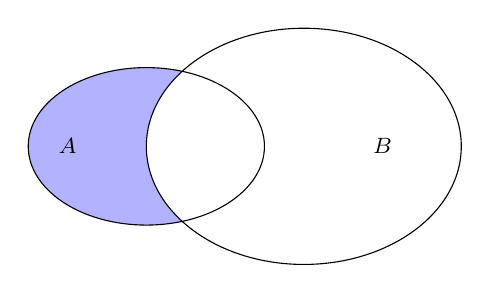
\begin{tikzpicture}[>=stealth,line join=round,line cap=round,font=\footnotesize,scale=1]
        \def\firstellipse{(0.5,0) ellipse (1.5 and 1)}
        \def\secondellipse{(2.5,0) ellipse (2 and 1.5)}
        \begin{scope}
            \clip \firstellipse ;
            \fill[blue!30] \firstellipse;
            \fill[white] \secondellipse;
        \end{scope}
        \draw \firstellipse \secondellipse;
        \node at (-0.5,0){$A$};
        \node at (3.5,0){$B$};
        
    \end{tikzpicture}
    \end{center}
    \choice
    {\True $A \setminus B$}
    {$A \cap B$}
    {$A \cup B$}
    {$B \setminus A$} 
    \loigiai
    {
        Phần gạch sọc trong hình vẽ là $A \setminus B$.
    }
\end{ex}



\Closesolutionfile{ans}
%\begin{center}
%	\textbf{ĐÁP ÁN}
%	\inputansbox{10}{ans/ans}	
%\end{center}
\begin{center}
	\textbf{PHẦN 2 - TỰ LUẬN}
\end{center}

\begin{bt}%[0D1Y3-1]%[0D1B3-2]%[Dự án đề kiểm tra HKII NH22-23-Nguyễn Tài Tuệ]%[THPT Chuyên Lê QUý Đôn- Quảng Trị] 
	  Cho hai tập hợp $A=\{x \in \mathbb{R},-4 \leq x<2\}$ và $B=[0 ; 4]$. Xác định các tập hợp sau  $A \cap B$, $A \cup B$, $B\setminus  A$.
	\loigiai{
		Ta có $ A=[-4;2) $, do đó 
		\begin{itemize}
			\item $A\cap B=[0;2).$
             \item $A\cup B=[-4;4].$
             \item $B \setminus A=[2;4].$ 
		\end{itemize}
	}
\end{bt}

\begin{bt}%[0X1B3-4] %[Dự án đề kiểm tra HKII NH22-23-Nguyễn Tài Tuệ]%[THPT Chuyên Lê QUý Đôn- Quảng Trị] 
  Có $ 100 $ học sinh tham dự kì thi học sinh giỏi Toán (thang điểm $ 20 $). Kết quả cho trong bảng sau 
  \begin{center}
  	 \begin{tabular}{|c|c|c|c|c|c|c|c|c|c|c|c|}
  	 	\hline Điểm & 9 & 10 & 11 & 12 & 13 & 14 & 15 & 16 & 17 & 18 & 19 \\
  	 	\hline Số học sinh & 1 & 1 & 3 & 5 & 8 & 13 & 19 & 24 & 14 & 10 & 2 \\
  	 	\hline
  	 \end{tabular}
  \end{center}	
	Tìm số trung bình, trung vị, các tứ phân vị và mốt của các số liệu trên  ( Yêu cầu ghi cụ thể cách xác định trung vị, các tứ phân vị).
	\loigiai{
		Giá trị trung bình $ \overline{x}=15{,}23 $.\\
		Do có $ 100 $ số liệu nên trung vị là trung bình cộng của số liệu thứ $ 50 $ và $ 51 $ sau khi đã xếp số liệu theo thứ tự không giảm ta có $M_e=\dfrac{15+16}{2}=15,5$.\\
		Các tứ phân vị\begin{itemize}
			\item $Q_2=M_{e}=15,5$.
			\item 	$Q_1$ là trung vị của $ 50 $ số liệu đầu nên nó là trung bình cộng của số liệu thứ $ 25 $ và $26$  nên $ Q_1=\dfrac{14+14}{2}=14$.\\
			\item $Q_3$ là trung vị của $ 50 $ số liệu sau nên nó là trung bình cộng của số liệu thứ $ 75 $ và $ 76 $ nên $Q_3=\dfrac{17+17}{2}=17$.
		\end{itemize}  
	 
		Mốt $M_o=16$.
	}
\end{bt}

\begin{bt}%[0H3K2-3]%[Dự án đề kiểm tra HKII NH22-23-Nguyễn Tài Tuệ]%[THPT Chuyên Lê QUý Đôn- Quảng Trị] 
	 Cho tam giác $ABC$. Gọi $M$, $N$ là trung điểm $AB$, $BC$ và $P$ là điểm thỏa mãn $\overrightarrow{AP}=2 \overrightarrow{PC}$.
	 \begin{enumerate}
	 	\item  Chứng minh rằng $\overrightarrow{M P}=-\dfrac{1}{2}\overrightarrow{A B}+\dfrac{2}{3}\overrightarrow{A C}$.
	 	\item Biết $AB=3a$; $AC=6 a$, $A=60^{\circ}$. Tính $\left |\overrightarrow{M N}+\overrightarrow{MP}\right |$.
	 \end{enumerate}
 \loigiai{
 	\begin{center}
 		 \begin{tikzpicture}
 		 	\path
 		 	(0,0) coordinate (A)
 		 	(4,0) coordinate (C)
 		 	(1.5,2) coordinate (B)
 		 	($ (A)!0.5!(B) $) coordinate (M)
 		 	($ (B)!0.5!(C) $) coordinate (N)
 		 	($ (A)!2/3!(C) $) coordinate (P)
 		 	($ (A)!7/6!(C) $) coordinate (F)
 		 	($ (A)!-1/2!(B) $) coordinate (E)
 		 	($ (E)+(F)-(A) $) coordinate (K)
 		 	;
 		 	\draw(A)--(B)--(C)--cycle (A)--(E)--(K)--(F)--(C) (A)--(K) (M)--(P) ;
 		 	\foreach \p/\g in {A/180,B/90,C/80,M/180, N/0,P/-90,F/90,E/180,K/-90} \draw[fill] (\p) circle(.5pt)node [shift={(\g:.35)}] {$\p$};
 		 \end{tikzpicture}
 	\end{center}
 	
 \begin{enumerate}
 	\item Ta có $\overrightarrow{MP}=\overrightarrow{AP}-\overrightarrow{AM}=-\dfrac{1}{2}\overrightarrow{AB}+\dfrac{2}{3}\overrightarrow{AC}$.
 	\item Theo giả thiết, ta có\\ $\left |\overrightarrow{MN}+\overrightarrow{MP}\right |=\left|\dfrac{1}{2}\overrightarrow{AC}+\left(-\dfrac{1}{2}\overrightarrow{AB}+\dfrac{2}{3}\overrightarrow{AC}\right)\right|=\left|-\dfrac{1}{2}\overrightarrow{AB}+\dfrac{7}{6}\overrightarrow{AC}\right|$.\\
 	Dựng điểm $ E $ đối xứng với $ M $ qua $ A $ và dựng điểm $ F $ sao cho $\overrightarrow{AF}=\dfrac{7}{6}\overrightarrow{AC}$ và điểm $ K $ sao cho $ AEKF $ là hình bình hành.\\
 	Ta có
 	$ \left|-\dfrac{1}{2}\overrightarrow{AB}+\dfrac{7}{6}\overrightarrow{AC}\right|   =\left |\overrightarrow{AE}+\overrightarrow{AF}\right |=\left |\overrightarrow{AK}\right |=AK$.\\
 	Ta có $ AE=\dfrac{1}{2}AB =\dfrac{3a}{2}$ và $ EK=AF=\dfrac{7}{6}AC =7a$,  $ \widehat{AEK} =60^\circ$.\\
 	Áp dụng đinh lí cô-sin vào tam giác $ AEK $ có\\
 	$ AK^2=AE^2+EK^2-2AE\cdot EK\cdot \cos \widehat{AEK} =\left(\dfrac{3a}{2}\right)^2+\left(7a\right)^2-2\cdot \dfrac{3a}{2}\cdot7a\cdot\dfrac{1}{2}=\dfrac{163a^2}{4}$\\
 	$ \Rightarrow AK=\dfrac{a\sqrt{163}}{2}  $.\\
 	Vậy $\left |\overrightarrow{MN}+\overrightarrow{MP}\right |=\dfrac{a\sqrt{163}}{2}$.
 	
 \end{enumerate}
 }
\end{bt}

\begin{bt}%[0H3K2-4]%[0H3K2-5]%[Dự án đề kiểm tra HKII NH22-23-Nguyễn Tài Tuệ]%[THPT Chuyên Lê QUý Đôn- Quảng Trị] 
	  Trong mặt phẳng tọa độ $Oxy$, cho hình chữ nhật $ABCD$. Kẻ $BH \perp AC ~(H \in AC)$. Gọi $M$, $N$ lần lượt là trung điểm của $AH$ và $DC$. Biết $M(11; 12)$, $N(10 ; 5)$, $H(17 ; 4)$.
	  \begin{enumerate}
	  	\item Tìm tọa độ điểm $A$ và tính diện tích tam giác $HMN$.
	  	\item  Tìm tọa độ điểm $B$.
	  \end{enumerate}
	 \loigiai{
	 	\begin{center}
	 	
	  \begin{tikzpicture}
	  	\path
	  	(0,0)  coordinate (D)
	  	(4,0) coordinate (C)
	  	(4,3) coordinate (B)
	  	(0,3) coordinate (A)
	  	($ (A)!(B)!(C)$) coordinate (H)
	  	($ (A)!0.5!(H) $) coordinate (M)
	  	($ (D)!0.5!(C) $) coordinate (N)
	  	;
	  	\draw (A)--(B)--(C)--(D)--cycle (A)--(C) (H)--(B)--(M)--(N) --(H);
	  	\foreach \p/\g in {A/90,B/90,C/-90,D/-90,M/-150,N/-90,H/100} \draw[fill] (\p) circle(.5pt)node [shift={(\g:.3)}] {$\p$};
	  \end{tikzpicture}  	 
\end{center}
 
	 	\begin{enumerate}
	 		\item Ta có $\overrightarrow{M A}\left(x_A-11 ; y_A-12\right)=\overrightarrow{H M}(-6 ; 8) \Rightarrow A(5 ; 20)$.\\
	 		Suy ra    $MN=\sqrt{(10-11)^2+(5-12)^2}=\sqrt{50}$, $NH=\sqrt{(17-10)^2+(4-5)^2}=\sqrt{50}$, $MH=\sqrt{(17-11)^2+(4-12)^2}=10$. \\
	 		Sử dụng công thức Hê-rông, diện tích tam giác $ HMN $  ta có \\
	 		 $ S=\sqrt{p\cdot (p-MN)(p-MH)(p-HN)}=25 $, với $ p=\dfrac{MN+NH+HN}{2}. $  
	 		\item Ta có 
	 		\begin{eqnarray*}
	 			 \overrightarrow{B M} \cdot \overrightarrow{M N}
	 			 &=&\dfrac{1}{2}\left (\overrightarrow{B A}+\overrightarrow{B H}\right )\left (\overrightarrow{M C}+\overrightarrow{C N}\right  )=\dfrac{1}{2}\left (\overrightarrow{B A} \cdot \overrightarrow{M C}+\overrightarrow{B A} \cdot \overrightarrow{C N}+\overrightarrow{B H} \cdot \overrightarrow{C N}\right ) \\ & =&\dfrac{1}{2}\left(\overrightarrow{B A} \cdot \overrightarrow{M C}+\dfrac{1}{2} \overrightarrow{B A} \cdot \overrightarrow{B A}+\dfrac{1}{2} \overrightarrow{B H} \cdot \overrightarrow{B A}\right)=\dfrac{1}{2} \overrightarrow{B A}\left (\overrightarrow{M C}+\overrightarrow{B M}\right )\\
	 			 &=&\dfrac{1}{2} \overrightarrow{B A} \cdot \overrightarrow{B C}=0.
	 		\end{eqnarray*}
 		 Gọi $B(a ; b)$. Ta có 
 		 $$
 		\heva{& \vec { H B } \cdot \vec { M H } = 0   \\
 		 	& \vec { M B } \cdot \vec { M N } = 0 }
 		\Leftrightarrow \heva{
 		 	 & 6 ( a - 1 7 ) - 8 ( b - 4 ) = 0   \\
 		 	& - ( a - 1 1 ) - 7 ( b - 1 2 ) = 0  
 	} \Leftrightarrow \heva{
 		 	&a=25 \\
 		 &	b=10.} $$
 		 Vậy $B(25 ; 10)$.
	 		 
	 	\end{enumerate}
	 }
\end{bt}


